\documentclass[tikz,border=10pt]{standalone}
\usetikzlibrary{shapes,arrows,positioning,calc,fit,backgrounds}
\usepackage{amsmath,amssymb}

\begin{document}
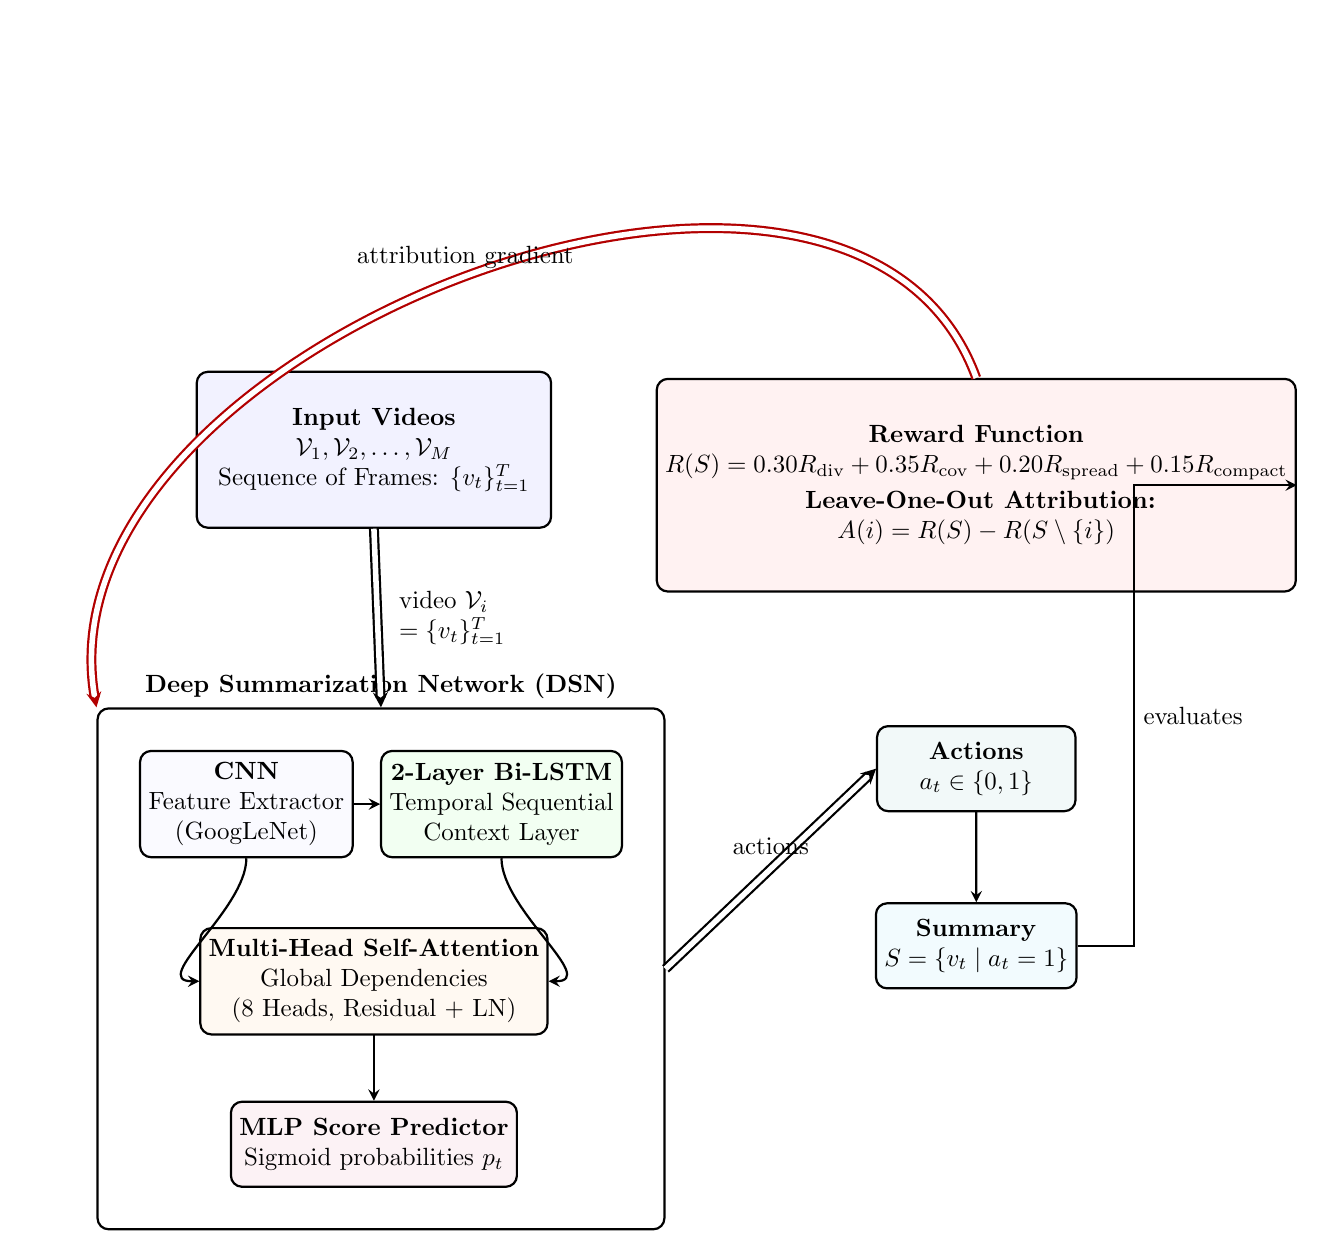
\begin{tikzpicture}[
    scale=0.9, every node/.style={transform shape},
    box/.style={draw, rectangle, rounded corners, minimum width=2.8cm, minimum height=1.5cm, align=center, thick},
    container/.style={draw, rectangle, rounded corners, inner sep=15pt, thick},
    arrow/.style={->, >=stealth, thick},
    doublearrow/.style={->, >=stealth, double, double distance=2pt, thick},
    line/.style={thick}
]

    % 1. Videos (Top Left)
    \node[box, fill=blue!5!white, minimum width=5cm, minimum height=2.2cm] (videos) at (0, 5) {
        \textbf{Input Videos} \\
        $\mathcal{V}_1, \mathcal{V}_2, \dots, \mathcal{V}_M$ \\
        Sequence of Frames: $\{v_t\}_{t=1}^T$
    };

    % 2. DSN Container (Bottom Left)
    \node[box, fill=blue!2!white, minimum width=3cm, minimum height=1.5cm] (cnn) at (-1.8, 0) {
        \textbf{CNN} \\
        Feature Extractor \\
        (GoogLeNet)
    };
    
    \node[box, fill=green!5!white, minimum width=3.2cm, minimum height=1.5cm] (bilstm) at (1.8, 0) {
        \textbf{2-Layer Bi-LSTM} \\
        Temporal Sequential \\
        Context Layer
    };

    \node[box, fill=orange!5!white, minimum width=4.5cm, minimum height=1.5cm] (mhsa) at (0, -2.5) {
        \textbf{Multi-Head Self-Attention} \\
        Global Dependencies \\
        (8 Heads, Residual + LN)
    };

    \node[box, fill=purple!5!white, minimum width=4cm, minimum height=1.2cm] (mlp) at (0, -4.8) {
        \textbf{MLP Score Predictor} \\
        Sigmoid probabilities $p_t$
    };

    % Fit container around DSN components
    \node[container, label=above:\textbf{Deep Summarization Network (DSN)}] (dsn) [fit=(cnn) (bilstm) (mhsa) (mlp)] {};

    % 3. Reward Function Container (Top Right)
    \node[box, fill=red!5!white, minimum width=7.2cm, minimum height=3.0cm] (reward) at (8.5, 4.5) {
        \textbf{Reward Function} \\
        $R(S) = 0.30 R_{\text{div}} + 0.35 R_{\text{cov}} + 0.20 R_{\text{spread}} + 0.15 R_{\text{compact}}$ \\
        \rule{0pt}{2.5ex} \textbf{Leave-One-Out Attribution:} \\
        $A(i) = R(S) - R(S \setminus \{i\})$
    };

    % 4. Actions & Summary (Middle Right)
    \node[box, fill=teal!5!white, minimum width=2.8cm, minimum height=1.2cm] (actions) at (8.5, 0.5) {
        \textbf{Actions} \\
        $a_t \in \{0,1\}$
    };
    
    \node[box, fill=cyan!5!white, minimum width=2.8cm, minimum height=1.2cm] (summary) at (8.5, -2.0) {
        \textbf{Summary} \\
        $S = \{v_t \mid a_t = 1\}$
    };

    % 5. Connections
    \draw[doublearrow] (videos.south) -- node[right, xshift=5pt, align=left] {video $\mathcal{V}_i$ \\ $= \{v_t\}_{t=1}^T$} (dsn.north);
    \draw[arrow] (cnn) -- (bilstm);
    \draw[arrow] (bilstm.south) to[out=270, in=0] (mhsa.east);
    \draw[arrow] (cnn.south) to[out=270, in=180] (mhsa.west);
    \draw[arrow] (mhsa) -- (mlp);
    
    \draw[doublearrow] (dsn.east) -- node[above, yshift=2pt] {actions} (actions.west);
    \draw[arrow] (actions) -- (summary);
    
    % Route summary to reward around actions box
    \draw[arrow] (summary.east) -- ++(0.8,0) |- node[right, pos=0.25] {evaluates} (reward.east);
    
    % Feedback loop arching over top of videos
    \draw[doublearrow, red!70!black] (reward.north) to[out=110, in=100] node[above, black] {attribution gradient} (dsn.north west);

\end{tikzpicture}
\end{document}
